{\color{indiagreen}\subsection{Sila}}
\textbf{Učinki sil}:
\begin{itemize}
	\item SPREMEMBE GIBANJA(ustavi, sprememba hitrosti, smeri...)
	\item DEFORMACIJA(sprememba oblike)
\end{itemize}
\textbf{SILE}:
\begin{itemize}
	\item NOTRANJE(med deli opazovanega telesa)
	\item ZUNANJE(s katerimi predmeti iz okolice delujemo na opazovalno telo)
\end{itemize}
\textbf{SEŠTEVANJE SIL}:
\begin{itemize}
	\item PARALELOGRAMSKO PRAVILO(premaknemo v izhodišče in naredimo vzporednice(paralelogram))
	\begin{center}
		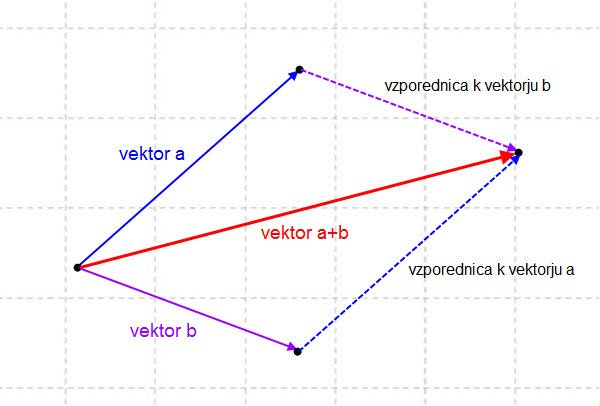
\includegraphics[width=16cm, height=9cm,keepaspectratio=true]{paralelogramsko_pravilo.jpg}
	\end{center}
	\item TRIKOTNIŠKO PRAVILO(silo premaknemo na konce prve sile)
	\begin{center}
		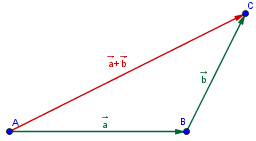
\includegraphics[width=8cm, height=5cm,keepaspectratio=true]{trikotnisko_pravilo.png}
	\end{center}
\end{itemize}
\textbf{RASTAVLJANJE SIL}
%\begin{center}
%	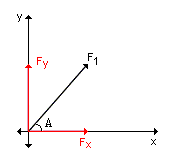
\includegraphics[width=16cm, height=9cm,keepaspectratio=true]{rastavljanje_sil.jpg}
%\end{center}